To create a TikZ LaTeX diagram that represents the update functions of a Boolean network and its uncontrolled synchronous dynamics, we can use a combination of nodes and edges to form the binary trees. Here's an example code snippet:
```
\documentclass{article}
\usepackage{tikz}
\begin{document}
\begin{figure}[h]
    \centering
    \begin{tikzpicture}[level distance=2cm,
        level 1/.style={sibling distance=4cm},
        level 2/.style={sibling distance=2cm}]
        % Left tree for update functions
        \node {Update Functions}
            child {node {000}}
            child {node {001}}
            child {node {010}}
            child {node {011}}
            child {node {100}}
            child {node {101}}
            child {node {110}}
            child {node {111}};
        % Right tree for uncontrolled synchronous dynamics
        \node[right=3cm] {Uncontrolled Synchronous Dynamics}
            child {node {000}}
            child {node {001}}
            child {node {010}}
            child {node {011}}
            child {node {100}}
            child {node {101}}
            child {node {110}}
            child {node {111}};
    \end{tikzpicture}
    \caption{Update functions of the Boolean network and its uncontrolled synchronous dynamics}
    \label{fig:boolean-network-update-functions}
\end{figure}
```
This code creates two binary trees side by side, one representing the update functions and the other representing the uncontrolled synchronous dynamics. Each tree has eight nodes, corresponding to the possible combinations of three binary digits. The `level distance` option controls the vertical spacing between levels of the tree, while the `sibling distance` option controls the horizontal spacing between sibling nodes.
You can customize this code further to add labels, arrows, and other elements to better illustrate the hierarchical structure and flow of the Boolean network.